\selectlanguage{ngerman}%
\frenchspacing%
\begin{ledgroupsized}[r]{120mm}%
\footnotesize%
\pstart%
\noindent\textbf{Überlieferung:}%
\pend%
\end{ledgroupsized}%
\begin{ledgroupsized}[r]{114mm}%
\footnotesize%
\pstart%
\parindent -6mm%
\makebox[6mm][l]{\textit{L}}%
Aufzeichnung:
LH~XXXV~11,\;14 Bl.\;3\textendash4. 
Ein Bogen~4\textsuperscript{o},
oberer Rand beschnitten.
\href{\Scan{LH_35_11_14_003-004wz}}{Gegenmarke} eines Wasserzeichens im Falz.
Vier Seiten. %
Ein Kustos am Ende von N.\;\ref{58940} %
verweist auf N.\;\ref{58939}.%
\pend%
\end{ledgroupsized}%
\selectlanguage{latin}%
\frenchspacing%
\vspace{8mm}
\count\Bfootins=1000
\count\Afootins=1200
\count\Cfootins=1000
\pstart%
\normalsize%
\noindent%
\lbrack%
\href{\Scan{LH_35_11_14_003r}}%
{3\,r\textsuperscript{o}}%
\rbrack%
\phantom{Ult.\;Octob.\;1690}%
\hfill%
\phantom{\lbrack3\,r\textsuperscript{o}\rbrack}%
Ult.\;Octob.\;1690%
\edtext{}{%
\lemma{\textit{Am oberen Rand:}}\Afootnote%
{%
Videantur quae ascripsimus pag.\;3 signo NB NB.\textsuperscript{\lbrack a\rbrack}%
\indexS{signum}
\\[1ex]%
{\footnotesize%
\textsuperscript{\lbrack a\rbrack}~NB NB:
Siehe die Randbemerkung zu \refpassage{35_11_14_003v_rndbmrkng-1}{35_11_14_003v_rndbmrkng-2}
(in \textit{L} am Rand von Bl.\;4\,r\textsuperscript{o},
bezogen auf Bl.\;3\:v\textsuperscript{o}).%
}}}%
\pend%
\pstart%
\noindent%
\centering%
De impulsu Eccentrico%
\indexS{impulsus eccentricus}
scheda 2\textsuperscript{a}%
\indexS{scheda}%
\edtext{}{%
\lemma{\textit{Am Rand:}}\Afootnote{%
Sub finem\textsuperscript{\lbrack a\rbrack}%
\indexS{finis}
rem videor assecutus per collationem diversarum virium respectivarum.%
\indexS{collatio virium respectivarum}%
\indexS{vis respectiva}%
\\[1ex]%
{\footnotesize%
\textsuperscript{\lbrack a\rbrack}~Sub finem:
Siehe \refpassage{LH_35_11_14_004v_subfinem-1}{LH_35_11_14_004v_subfinem-2}.%
}}}
\pend%
\vspace{0.5em}%
\pstart%
\noindent%
\edlabel{LH_35_11_14_003-004_003r_methodus-1}%
Perjudiciale experimentum%
\indexS{experimentum perjudicale}
sumendum esset;
si \textit{A} incurrat in \textit{B}%
\indexS{corpus incurrens}%
\indexS{incursus eccentricus}
connexum cum \textit{C},%
\indexS{corpora connexa}
utrum reflectatur perinde%
\indexS{corpus reflexum}%
\indexS{reflexio corporis incurrentis}
ac si solum incurrisset in \textit{B},
licet \textit{B} deinde impulsu%
\indexS{impulsus eccentricus}
suo abripiat \textit{C}.%
\indexS{corpus abreptum}%
\indexS{abreptio corporis impulsi}%
\edlabel{LH_35_11_14_003-004_003r_methodus-2}
Quid autem hoc posito fiat,
ita explicemus distinctius:
\edlabel{LH_35_11_14_003r_aequales-1}%
ponamus \textit{A}, \textit{B}, \textit{C} esse aequales,%
\indexS{corpora aequalia}%
\edlabel{LH_35_11_14_003r_aequales-2}
et\;\textit{A} incurrere in \textit{B}%
\indexS{corpus incurrens}%
\indexS{incursus eccentricus}
celeritate 1.%
\indexS{celeritas incursus}
Utique quiescet in loco incursus,%
\indexS{locus incursus}%
\indexS{quies post incursum}
et deinde \textit{B} perget eadem celeritate
quam habuit \textit{A}.%
\indexS{celeritas incursus}
Jam \textit{B}
\edtext{inciden\lbrack te\rbrack%
\indexS{corpus incidens in vinculum}%
}{%
\lemma{incidens}\Bfootnote{%
\textit{L~ändert Hrsg.}}}
in vinculum \textit{CB}%
\indexS{vinculum}
quo ipsi \textit{C} connectitur%
\indexS{corpora connexa}%
\lbrack,\rbrack\
ad angulos rectos%
\indexS{angulus rectus}%
\lbrack,\rbrack\
quid
\edtext{\lbrack fiat\rbrack}{%
\lemma{fiat}\Bfootnote{%
\textit{erg. Hrsg.}}}
facile ita explicabimus,
primum considerando communem motum centri gravitatis%
\indexS{centrum gravitatis commune}%
\indexS{motus centri gravitatis}%
\lbrack,\rbrack\
isque perget ut ante,
et reliquum deinde motum privatum%
\indexS{motus privatus}%
\indexS{motus reliquus}
seu respectivum%
\indexS{motus respectivus}
qui convertetur in gyrationem%
\indexS{motus conversus in gyrationem}
circa centrum.%
\indexS{centrum gravitatis commune}%
\indexS{gyratio circa centrum gravitatis}%
\pend%
\begin{edfigure}[2.00em][0.00em]%
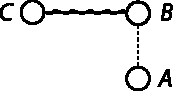
\includegraphics[width=0.19\textwidth]{gesamttex/edit_VIII-4/images/LH_35_11_14_003-004_d01_003r.pdf}%
\edcaption[0.50em]%
{%
\lbrack\textit{Fig.\:1}\rbrack%
}%
\end{edfigure}%
\newpage%
\begin{edfigure}[0.00em][1.50em]%
\vspace*{0.0em}%
\hspace{-85mm}%
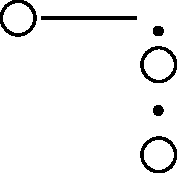
\includegraphics[width=0.11\textwidth]{gesamttex/edit_VIII-4/images/LH_35_11_14_003-004_d02_003r.pdf}%
\edcaption[0.25em]%
{%
\hspace{-85mm}%
\lbrack\textit{Fig.\:2, gestr.}\rbrack%
}%
\vspace{-6,5em}%
\hspace{85mm}%
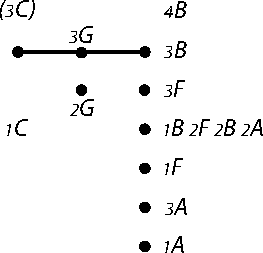
\includegraphics[width=0.20\textwidth]{gesamttex/edit_VIII-4/images/LH_35_11_14_003-004_d03_003r.pdf}%
\edcaption[0.25em]%
{%
\hspace{85mm}%
\lbrack\textit{Fig.\:3, gestr.}\rbrack%
\edtext{}{\lemma{\lbrack\textit{Fig.\:3}\rbrack}%
\Cfootnote[nonum]{%
Hierzu liegt in \textit{L} ein gestr., nicht wiedergegebener Entwurf vor.%
}}%
\edtext{}{%
\lemma{\textit{Unter%
} \lbrack\textit{Fig.\:3}\rbrack:%
}%
\Afootnote[nonum]{%
\quad%
$\ind{1}F\ind{2}F
=
\ind{2}F\ind{3}F
=
FB.$
\quad%
$\ind{2}B\ind{3}B
=
\text{bis}\ FB.$
\quad%
$\ind{2}A\ind{3}A
=
FA - FB.$%
}}%
}%
\vspace{0.25em}%
\includegraphics[width=0.40\textwidth]{%
gesamttex/edit_VIII-4/images/LH_35_11_14_003-004_d04_003r.pdf}%
\edcaption[0.25em]%
{%
\lbrack\textit{Fig.\:4}\rbrack%
}%
\end{edfigure}%
\pstart%
Sit
\edtext{\textit{F} centrum gr.%
\indexS{centrum gravitatis commune}%
}{%
\lemma{\textit{F} cen\-trum gr.\,}\Cfootnote{%
Vgl. das Diagramm \lbrack\textit{Fig.\:4}\rbrack.%
}}
inter \textit{A} et \textit{B}.
$\ind{1}F\ind{2}F
=
\ind{2}F\ind{3}F.$
Coincidunt
\textit{\ind{1}B},\;%
\textit{\ind{2}B},\;%
\edtext{\lbrack\textit{\ind{2}F}\rbrack,}{%
\lemma{\textit{\ind{2}B}}\Bfootnote{%
\textit{L~ändert Hrsg.}}}%
\;%
\textit{\ind{2}A}
(\protect\vphantom)%
si sumamus corpora ut puncta%
\indexS{corpus sumptum ut punctum}%
\protect\vphantom().
$\ind{3}F\ind{3}B
=
\ind{1}F\ind{1}B$
et
\edtext{%
$\ind{2}F\ind{3}A
=
\ind{1}F\ind{1}A,$%
}{%
\lemma{$\ind{3}F\ind{3}A
=
\ind{1}F\ind{1}A$\,%
}\Cfootnote{%
Die Bedingung $A = B = C$ (vgl. \refpassage{LH_35_11_14_003r_aequales-1}{LH_35_11_14_003r_aequales-2}) gilt jetzt nicht mehr.
Sonst müsste unter der Annahme, dass der Körper \textit{B} vor dem Stoß ruht, an dessen Stelle der Körper \textit{A} nach dem Stoß in \textit{\ind{2}A} ruhen.%
}}
adeoque
\edtext{%
$\ind{1}A\ind{1}B
=
[\ind{3}A\ind{3}F].$ %
$\ind{2}B\ind{3}B
=
\ind{2}F\ind{3}F
+
\ind{3}F\ind{3}B
=
\ind{1}F\ind{2}F
+
\ind{1}F\ind{1}B.\
\ind{2}B\ind{3}B
=
\text{bis}\
\ind{1}F\ind{2}F$
seu bis \textit{FB}.
$\ind{2}A\ind{3}A
=
FA - FB.$
Jam \textit{B} in \textit{\ind{3}B} %
incidat in vinculum%
\indexS{corpus incidens in vinculum}%
\indexS{vinculum}
quod%
}{%
\lemma{$\ind{1}A\ind{1}B =$}\Bfootnote{%
\bars{$\ind{3}A\ind{3}B$ \textit{ändert Hrsg.}}.
\textit{(1)}~Jam \textit{\ind{3}B} incidat in vinculum quo
\textit{(2)}~$\ind{2}B\ind{3}B = \ind{2}F \ind{3}F \, +$ %
\lbrack...\rbrack\ vinculum quod%
~\textit{L}}}
ipsum connectat cum%
\indexS{corpora connexa}
\edtext{\lbrack\textit{C}\rbrack.}{%
\lemma{\textit{B}}\Bfootnote{%
\textit{L~ändert Hrsg.}}}
In situ%
\indexS{situs}
\textit{\ind{2}BC}
erat centrum gravitatis
\textit{\ind{2}G};%
\indexS{centrum gravitatis commune}
in situ%
\indexS{situs}
\textit{\ind{3}BC}
erat
\textit{\ind{3}G};
rectaque
\textit{\ind{2}G\ind{3}G}
parallela ipsi
\textit{\ind{2}B\ind{3}B}.
Et hoc perget
eadem celeritate%
\indexS{celeritas centri gravitatis}
et directione%
\indexS{directio centri gravitatis}
in \textit{\ind{4}G}.
Cum autem cohaereant \textit{B} et \textit{C},%
\indexS{corpora cohaerentia}
vis eorum respectiva%
\indexS{vis respectiva}
vertetur in%
\indexS{vis versa in circulationem}
\edlabel{35_11_14_003-004_1a}%
circulationem.%
\indexS{circulatio in concursu eccentrico}%
\edtext{}{%
\xxref{35_11_14_003-004_1a}{35_11_14_003-004_1b}%
\lemma{circulationem.}\Bfootnote{%
\textit{(1)}~Quod
\textit{(2)}~Est autem motus duplex
\textit{(3)}~Potest enim \lbrack...\rbrack\ duplici componi,%
~\textit{L}}}
Potest enim motus ex duplici componi,%
\indexS{motus compositus}%
\edlabel{35_11_14_003-004_1b}
ex communi%
\indexS{motus communis}
centri gravitatis,%
\indexS{centrum gravitatis commune}%
\indexS{motus centri gravitatis}
qui est celeritatis
\textit{\ind{2}G\ind{3}G}%
\indexS{celeritas centri gravitatis}
ductae in
$B + C,$
et proprio contrario%
\indexS{motus proprius}%
\indexS{motus contrarius}
\edtext{%
reciproco.%
\indexS{motus proprius}%
\indexS{motus reciprocus}
Jam celeritas%
}{\lemma{reciproco.}\Bfootnote{%
\textit{(1)}~, qui \textlangle\textendash\textrangle\ in
\textit{(2)}~. Jam celeritas%
~\textit{L}}}
quam dederamus ipsi \textit{B} %
\edtext{erat
\textit{\ind{2}B\ind{3}B},
et}{%
\lemma{erat}\Bfootnote{%
\textit{\ind{2}B\ind{3}B},
\textit{(1)}~ergo
\textit{(2)}~et%
~\textit{L}}}
\textit{\ind{2}G\ind{3}G}
ad
\textit{\ind{2}B\ind{3}B}
ut
\textit{B} ad
\edtext{%
$B + C,$
et celeritas propria%
\indexS{celeritas propria}%
}{%
\lemma{$B + C,$}\Bfootnote{%
et
\textit{(1)}~motus proprio
\textit{(2)}~celeritas propria%
~\textit{L}}}
ipsius \textit{B}
erit
$\ind{2}B\ind{3}B
-
\ind{2}G\ind{3}G$
(\protect\vphantom)%
quia quiescit \textit{C}%
\indexS{corpus quiescens}%
\protect\vphantom()
seu ad
\textit{\ind{2}B\ind{3}B}
ut \textit{C}
ad $B + C,$
ut celeritas %
contraria%
\indexS{celeritas contraria}
est
$= \ind{2}G\ind{3}G$
seu est ad
\textit{\ind{2}B\ind{3}B}
ut \textit{B}
ad $B + C.$
Cum ergo velocitates hae respectivae%
\indexS{velocitas respectiva}
sint inter se ut corpora
\edtext{%
reciproce
et convertantur in
gyratio\lbrack nem\rbrack,%
\indexS{gyratio in concursu eccentrico}%
\indexS{velocitas conversa in gyrationem}
cum alia ratione%
\indexS{ratio alia}
praestari posse non appareat,
fiet gyratio circa centrum gravitatis,%
\indexS{gyratio circa centrum gravitatis}%
\indexS{centrum gravitatis commune}%
}{%
\lemma{reciproce}\Bfootnote{%
\textit{(1)}~ut convertantur in gyrationem circa \textit{G}
\textit{(2)}~et convertantur in
\bars{gyratio, \textit{ändert Hrsg.}},
cum alia %
\lbrack...\rbrack\ centrum gravitatis,%
~\textit{L}}}
et arcus
\textit{(\ind{3}B)\ind{4}B}%
\indexS{arcus circuli}
celeritatem gyrationis%
\indexS{celeritas gyrationis}
ipsius \textit{B} exprimens
erit aequalis priori velocitati respectivae ipsius \textit{B},%
\indexS{velocitas respectiva}
adeoque ad
\textit{\ind{2}B\ind{3}B}
ut \textit{C}
ad $B + C,$
\edtext{\lbrack et\rbrack}{%
\lemma{ut}\Bfootnote{%
\textit{L~ändert Hrsg.}}}
arcus
\textit{(\ind{3}C)\ind{4}C}%
\indexS{arcus circuli}
erit $=$
\textit{\ind{3}G\ind{4}G}
seu
\textit{\ind{2}G\ind{3}G},
et ita manebit velocitas respectiva.%
\indexS{velocitas respectiva}
Unde si liberarentur ambo simul in circulatione%
\indexS{circulatio in concursu eccentrico}%
\lbrack,\rbrack\
eandem quam ante velocitatem respectivam%
\indexS{velocitas respectiva}
retinerent pariterque communem.%
\indexS{velocitas communis}
Sed comparanda velocitas respectiva%
\indexS{velocitas respectiva}
inter \textit{A} et
\edtext{%
\textit{CB}, scil.
quaerenda est via centri gravitatis communis%
\indexS{centrum gravitatis commune}%
\indexS{via centri gravitatis}
omnium \textit{A}, \textit{B}, \textit{C}
seu ipsius \textit{H}.
Habetur autem punctum \textit{H} %
intersectione%
\indexS{intersectio rectarum}
rectarum \textit{AG} et\;\textit{FC}.%
}{%
\lemma{\textit{CB},}\Bfootnote{%
\textit{(1)}~prior scilicet
\textit{(a)}~\textit{A} ad
\textit{(b)}~ipsius \textit{A} accessio ad \textit{G}, cum quiesceret adhuc \textit{B}, erat \textit{\ind{1}A\ind{2}A}, sed mox recessus est $\ind{2}A\ind{3}A + \ind{2}G\ind{3}G,$ est autem 2.
\textit{(2)}~scil. quaerenda
\lbrack...\rbrack\ ipsius \textit{H}
\textit{(a)}~quo
\textit{(b)}~. Habetur autem
\lbrack...\rbrack\ \textit{AG} et \textit{FC}.%
~\textit{L}}}
\lbrack%
\href{\Scan{LH_35_11_14_003v}}%
{3\,v\textsuperscript{o}}%
\rbrack%
\pend%
\pstart%
Sed puto hanc Methodum non procedere,%
\indexS{methodus non procedens}
\edtext{vel centrici}{%
\lemma{vel}\Bfootnote{%
\textit{(1)}~singularis
\textit{(2)}~centrici%
~\textit{L}}}
concursus exemplo, %
\indexS{concursus centricus}
manifestum enim est
longe aliter reflecti%
\indexS{corpus incurrens}%
\indexS{corpus reflexum}%
\indexS{reflexio corporis incurrentis}
\edtext{%
\textit{A}
incurrens
in \textit{B},%
}{%
\lemma{\textit{A} incurrens in \textit{B}}\Cfootnote{%
Vgl. das Diagramm \lbrack\textit{Fig.\:5}\rbrack.}}
cum
\edtext{%
\textit{B} est sejuncta%
}{\lemma{\textit{B} est sejuncta}\Cfootnote{%
In dem vorliegenden und dem folgenden Absatz werden die zusammenstoßenden bzw. zusammenhängenden Körper %
abwechselnd mit dem Neutrum oder dem Femininum bezeichnet.%
}}
a \textit{C},%
\indexS{corpora sejuncta}
quam cum est continua.%
\indexS{corpora continua}
Interim
\edtext{putem servire casum disjuncti}{%
\lemma{putem}\Bfootnote{%
\textit{(1)}~hunc
\textit{(2)}~servire casum disjuncti%
~\textit{L}}}
ad casum continui investigandum,%
\indexS{casus corporum continuorum}
continue enim accedet%
\indexS{accessio continua}%
\lbrack;\rbrack\
et video revera eadem fieri,
sed cum nova accedit consideratio,%
\indexS{consideratio}
ut nempe ipsae \textit{B}, \textit{C}
non tantum sint continuae%
\indexS{corpora continua}%
\indexS{partes continuae}
sed et connexae,%
\indexS{corpora connexa}%
\indexS{partes connexae}
tum demum aliud eveniet.
Nempe ponamus
\textit{A}, \textit{B}, \textit{C} esse aequales%
\indexS{corpora aequalia}
et \textit{A} incidere in \textit{B},
quiescent \textit{A} et \textit{B},
movebitur \textit{C}.
Sed cum \textit{B} et \textit{C} sunt connexae%
\lbrack,\rbrack\
res sese longe aliter
\edlabel{35_11_14_003-004_2a}%
habet.%
\edtext{}{%
\xxref{35_11_14_003-004_2a}{35_11_14_003-004_2b}%
\lemma{habet}\Bfootnote{%
\textit{(1)}~quemadmodum
\lbrack/\rbrack\
\textit{(2)}~. Quemadmodum si
\textit{(3)}~. Regulae concursus centrici%
~\textit{L}}}%
\pend%
\pstart%
Regulae concursus centrici%
\edlabel{35_11_14_003-004_2b}%
\indexS{concursus centricus}%
\indexS{regula concursus centrici}
duorum%
\indexS{corpora concurrentia centrice}
\edtext{corporum \textit{a}, \textit{b}%
}{\lemma{corporum \textit{a}, \textit{b}%
}\Cfootnote{%
Vgl. das Diagramm \lbrack\textit{Fig.\:6}\rbrack.}}
debent esse tales
ut
circulantes%
\indexS{corpus circulans}
circa eundem axem \textit{LM}%
\indexS{axis circulationis}
et concurrentes
ac post concursum%
\indexS{concursus centricus}
reflexae,%
\indexS{corpus reflexum}
iterum ab altera parte
ob gyrum concurrentes%
\indexS{corpora concurrentia ob gyrum}%
\indexS{concursus ob gyrum}%
\indexS{gyrus post incursum}%
in \textit{(a)} et \textit{(b)}
restituant statum primum.%
\indexS{restitutio status primi}%
\indexS{status primus}
Idem et fieri debet in incursu eccentrico%
\indexS{incursus eccentricus}
ubi
\edtext{oritur progressus%
\indexS{progressus post incursum}
et gyrus,%
\indexS{gyrus post incursum}%
}{%
\lemma{oritur}\Bfootnote{%
\textit{(1)}~reflexio et gyrus
\textit{(2)}~progressus et gyrus,%
~\textit{L}}}
ut scilicet post concursum%
\indexS{concursus eccentricus}
oriatur simplex motus%
\indexS{motus simplex}
destructo gyro,%
\indexS{gyrus destructus}
debeat autem talis esse ambitus circuli gyrationis%
\indexS{gyratio in concursu eccentrico}%
\indexS{circulus gyrationis}%
\indexS{ambitus circuli gyrationis}
qui arbitrio potest assumi,%
\indexS{arbitrium}
ut sibi praecise rursus occurrant in eodem loco
saltem a latere opposito.
Pono autem concursus%
\indexS{concursus eccentricus}
initio esse proportionales ponderibus.%
\indexS{concursus proportionalis ponderibus}
Notandum etiam
\edtext{contra supradicta}{%
\lemma{contra supradicta}\Cfootnote{%
Möglicherweise N.\;\ref{58940}, \refpassage{LH_35_11_14_006r_sprdct-1}{LH_35_11_14_006r_sprdct-2}.%
}}%
\lbrack:\rbrack\
cum
\edtext{}{%
\xxref{LH_35_11_14_003v_corpusBC-1}{LH_35_11_14_003v_corpusBC-2}%
\lemma{corpus \textit{BC}}\Cfootnote{%
Vgl. das Diagramm \lbrack\textit{Fig.\:8}\rbrack.}}%
\edtext{%
\edlabel{LH_35_11_14_003v_corpusBC-1}%
corpus \textit{BC}%
\edlabel{LH_35_11_14_003v_corpusBC-2}
est in motu \textit{\ind{1}G\ind{2}G}%
}{%
\lemma{corpus}\Bfootnote{%
\textit{(1)}~\textit{B} agendum
\textit{(2)}~\textit{BC}
\textit{(a)}~agendum
\textit{(b)}~est in motu \textit{\ind{1}G\ind{2}G}%
~\textit{L}}}
et ab \textit{A} impellitur contrario itinere,%
\indexS{iter contrarium}
revera ipsum \textit{B} tantum,
non vero ipsum \textit{C} obstare gyro,%
\indexS{gyrus post incursum}
cum ita \textit{C} suum conatum%
\edlabel{35_11_14_003v_3a}
obtineat.%
\indexS{conatus obtentus}
\edtext{}{%
\xxref{35_11_14_003v_3a}{35_11_14_003v_3b}%
\lemma{obtineat.}\Bfootnote{%
\textit{(1)}~Manifestum est quatenus gyrus fit, eatenus rev
\textit{(2)}~Jam video
\lbrack...\rbrack\ ipso recedit.%
~\textit{L}}}%
\pend%
\pstart%
\edtext{}{%
\xxref{35_11_14_003v_rndbmrkng-1}{35_11_14_003v_rndbmrkng-2}%
\lemma{\textit{Quer am linken Rand von Bl.\;4\,r\textsuperscript{o}, mit Bezug auf Bl.\;3\,v\textsuperscript{o}:}}\Afootnote{%
NB NB
Hinc usque ad finem paginae 4%
\indexS{pagina}%
\textsuperscript{\lbrack a\rbrack}
per paginam sequentem%
\indexS{pagina}%
\textsuperscript{\lbrack b\rbrack}
videntur vera esse omnia,
nempe tribus modis diversis investigando
aequationem respectivarum potentiarum%
\indexS{aequatio potentiae respectivae}%
\indexS{potentia respectiva collecta cum totali}
collectarum cum totali.%
\indexS{potentia totalis collecta cum respectiva}
Res inchoanda a NB pag. sequentis.%
\indexS{pagina}%
\textsuperscript{\lbrack c\rbrack}
Imo adhuc ibi videtur in eo esse error,%
\indexS{error}
quod vis respectiva%
\indexS{vis respectiva}
non aestimanda solum in parallelis,
sed absolute quaerendo diminutionem distantiae.
Forte in hoc loco res non nocebit.
Altius tamen examinandum.%
\\[1ex]%
{\footnotesize%
\textsuperscript{\lbrack a\rbrack}~paginae 4\,:
Bl.\;4\,v\textsuperscript{o}.
\quad
\textsuperscript{\lbrack b\rbrack}~paginam sequentem\,:
Bl.\;4\,r\textsuperscript{o}.
\quad
\textsuperscript{\lbrack c\rbrack}~NB pag. sequentis\,:
Vgl. \refpassage{LH_35_11_14_004v_NB-1}{LH_35_11_14_004v_NB-2}.%
}}}%
\edlabel{35_11_14_003v_rndbmrkng-1}%
Jam video re recte considerata%
\lbrack:\rbrack\
quatenus fit gyrus%
\indexS{gyrus post ictum}
et quidem circa centrum gravitatis,%
\indexS{centrum gravitatis commune}
eatenus nullam habere locum celeritatem respectivam%
\indexS{celeritas respectiva corporis gyrantis}
corporis gyrantis,%
\indexS{corpus gyrans}
respectu alterius,
nam quantum unum ipsi accedit,
tantum alterum ab ipso recedit.%
\edlabel{35_11_14_003v_3b}
Caeterum gyratio%
\indexS{gyratio in concursu eccentrico}
debet fieri circa centrum%
\indexS{centrum gravitatis commune}
\edtext{gravitatis.
Ita enim \textit{B} et \textit{C} saltem}{%
\lemma{gravitatis.}\Bfootnote{%
\textit{(1)}~Alioqui
\textit{(2)}~Ita enim
\textit{(a)}~corpus a
\textit{(b)}~\textit{B} et \textit{C} saltem%
~\textit{L}}}
eandem retinent vim respectivam inter se,%
\indexS{vis respectiva}
nempe nullam,
ut ante.%
\edlabel{35_11_14_003v_rndbmrkng-2}%
\pend%
\vspace{1.0em} %
\centerline{%
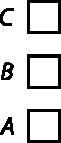
\includegraphics[width=0.066\textwidth]{gesamttex/edit_VIII-4/images/LH_35_11_14_003-004_d05_003v.pdf}}
\vspace{0.50em}
\centerline{%
\lbrack\textit{Fig.\:5}\rbrack}
\newpage
\vspace*{-0.0em} %
\centerline{\hspace{-70mm}%
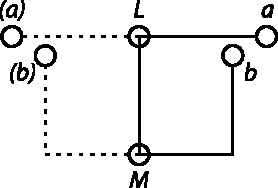
\includegraphics[width=0.30\textwidth]{gesamttex/edit_VIII-4/images/LH_35_11_14_003-004_d06_003v.pdf}}
\vspace{0.25em}
\centerline{\hspace{-70mm}%
\lbrack\textit{Fig.\:6}\rbrack}
\vspace{-8.6em} %
\centerline{\hspace{70mm}%
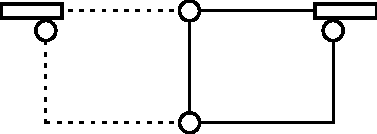
\includegraphics[width=0.425\textwidth]{gesamttex/edit_VIII-4/images/LH_35_11_14_003-004_d07_003v.pdf}}
\vspace{1.0em}
\centerline{\hspace{70mm}%
\lbrack\textit{Fig.\:7}\rbrack}
\vspace*{3.75em} %
\centerline{\hspace{-70mm}%
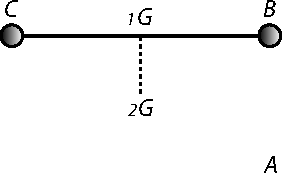
\includegraphics[width=0.30\textwidth]{gesamttex/edit_VIII-4/images/LH_35_11_14_003-004_d08_003v.pdf}}
\vspace{-0.5em}
\centerline{\hspace{-70mm}%
\lbrack\textit{Fig.\:8}\rbrack}
\vspace{-10.80em} %
\centerline{\hspace{70mm}%
\includegraphics[width=0.33\textwidth]{%
gesamttex/edit_VIII-4/images/LH_35_11_14_003-004_d09_003v.pdf}}
\vspace{1.0em}
\centerline{\hspace{70mm}%
\lbrack\textit{Fig.\:9}\rbrack}
\vspace{2.5em}
\pstart%
Verum quid
si contingat ipsa a connexione liberari?%
\indexS{connexio corporum}
Tunc magnam acquirent vim a se invicem recedendi,%
\indexS{vis recedendi}
ergo eam jam habent,
eaque
\edtext{intend\lbrack itur\rbrack}{%
\lemma{intendunt}\Bfootnote{%
\textit{L~ändert Hrsg.}}}
connectens%
\indexS{vis connectens}%
\lbrack;\rbrack\
praeterea vis%
\indexS{vis recedendi}
qua corpus \textit{A} recedit ab ipsorum centro gravitatis%
\indexS{centrum gravitatis commune}
etiam computanda est.
Et hae vires simul aequari debent potentiae respectivae%
\indexS{potentia respectiva}
quae initio
\edtext{fuit.
Sed tamen superest quaestio%
\indexS{quaestio}%
}{%
\lemma{fuit.}\Bfootnote{%
\textit{(1)}~Itaque
\textit{(2)}~ Sed quaeri
\textit{(3)}~Sed tamen superest quaestio%
~\textit{L}}}
quantus fieri debeat gyrus,%
\indexS{gyrus post ictum}
quanta vero progresssio%
\indexS{progressio post ictum}
seu reflexio.%
\indexS{reflexio post ictum}
\edtext{%
An dicemus corpora\;\textit{A} et\;\textit{B}
ob ictum%
\indexS{ictus}
a se invicem recedere%
\indexS{corpus recedens post ictum}%
\indexS{recessus post ictum}
celeritate%
\indexS{celeritas recessus}
qua advenere%
\indexS{celeritas adventus}%
\lbrack?\rbrack%
}{%
\lemma{dicemus}\Bfootnote{%
\textit{(1)}~corpus \textit{A} a corpore \textit{B} ea tantum recedere celeritate
\textit{(2)}~corpora \textit{A} 
\textit{(3)}~corpora \textit{A} %
\lbrack...\rbrack\ qua advenere.%
~\textit{L}}}
Nam inter
\edtext{ipsa}{%
\lemma{ipsa}\Bfootnote{%
\textit{erg.\;L}}}
sola fit ictus,%
\indexS{ictus}
cum oppositum
\edtext{\textit{C}}{%
\lemma{\textit{C}}\Bfootnote{%
\textit{erg.\;L}}}
non obstet,
sed progredi possit
non obstante impulsu%
\indexS{impulsus}
ipsius\;%
\edtext{%
\textit{B} versus\;\textit{L}.%
}{%
\lemma{\textit{B} versus \textit{L}}\Cfootnote{%
Vgl. das Diagramm \lbrack\textit{Fig.\:9}\rbrack.}}
Verum ut eadem in
\lbrack%
\href{\Scan{LH_35_11_14_004r}}%
{4\:r\textsuperscript{o}}%
\rbrack\ %
summa servetur vis respectiva%
\indexS{vis respectiva}
quae
\edtext{ante,
opus et gyro.}{%
\lemma{ante,}\Bfootnote{%
\textit{(1)}~id obtinetur gyro
\textit{(2)}~et ita oritur
\textit{(3)}~opus et gyro.%
~\textit{L}}}
Nam ictus%
\indexS{ictus}
non est nisi inter\;\textit{B} et\;%
\edtext{\lbrack\textit{A}\rbrack,}{%
\lemma{\textit{C}}\Bfootnote{%
\textit{L~ändert Hrsg.}}}
non potest autem eadem
\edtext{esse celeritas respectiva%
\indexS{celeritas respectiva}
inter\;\textit{A} et\;\textit{G}}{%
\lemma{esse}\Bfootnote{%
\textit{(1)}~vis respectiva inter \textit{B} et
\textit{(2)}~celeritas respectiva inter \textit{A} et \textit{G}%
~\textit{L}}}
quae ante,
alioqui nullus fieret gyrus,%
\indexS{gyrus post ictum}
qui et ipse novam vim respectivam continet.%
\indexS{vis respectiva}
Debet autem oriri
gyrus,%
\indexS{gyrus post ictum}
non
simplex recessus%
\indexS{recessus post ictum}
\edtext{seu regressus%
\indexS{regressus post ictum}%
}{%
\lemma{seu}\Bfootnote{%
\textit{(1)}~progressus
\textit{(2)}~regressus%
~\textit{L}}}
quia \textit{C} gyro%
\indexS{gyrus post ictum}
progressum suum%
\indexS{progressus post ictum}
\edtext{servat.
Quidni}{%
\lemma{servat.}\Bfootnote{%
\textit{(1)}~Quod si
\textit{(2)}~Quidni%
~\textit{L}}}
ergo solus erit gyrus?%
\indexS{gyrus post ictum}
Respondeo:
ita \textit{C} tenderet versus \textit{M}
celerius quam ante et nimis celeriter.
Videamus ergo
\edtext{an haec duo simul coincidant,
ut \textit{A} et \textit{B} eandem}{%
\lemma{an}\Bfootnote{%
\textit{(1)}~fiat
\textit{(2)}~haec duo simul coincidant, ut
\textit{(a)}~\textit{C} eand
\textit{(b)}~\textit{A} et \textit{B} eandem%
~\textit{L}}}
inter se servent velocitatem respectivam,%
\indexS{velocitas respectiva}
et ut \textit{C} eundem servet progressum;%
\indexS{progressus post ictum}
simulque ut efficiatur
ut summa eadem maneat vis respectiva.%
\indexS{vis respectiva}%
\pend%
\pstart%
Tentemus in exemplo:
sint
\edtext{\textit{A}, \textit{B}, \textit{C} aequales%
\indexS{corpora aequalia}%
}{%
\lemma{\textit{A}, \textit{B}, \textit{C} aequales}\Cfootnote{%
Vgl. das Diagramm \lbrack\textit{Fig.\:10}\rbrack.%
}}
et celeritas
(ex hypothesi)%
\indexS{hypothesis}
quantitatum reciproce proportionalis%
\indexS{celeritas reciproce proportionalis quantitati}
adeoque ipsius \textit{A} duplo major.
Jam si \textit{A} et \textit{B} ob ictum%
\indexS{ictus}
eadem a se invicem celeritate respectiva%
\indexS{celeritas respectiva}
resiliunt%
\indexS{corpus resiliens}%
\indexS{resilitio post ictum}
quam habuerunt,
ideo cum sint aequalia%
\indexS{corpora aequalia}%
\lbrack,\rbrack\
distantia%
\indexS{distantia corporum concurrentium}
prior \textit{\ind{1}B\ind{1}A} %
erit bisecanda in \textit{D},
et sumatur \textit{\ind{2}A\ind{3}A} %
aequalis ipsi \textit{D\ind{1}A},
quae erit reflexio ipsius \textit{A} ob ictum.%
\indexS{ictus}%
\indexS{reflexio ob ictum}
Jam \textit{\ind{2}B} habebit celeritatem tendendi retrorsum%
\indexS{celeritas tendendi retrorsum}
quae etiam sit ut \textit{\ind{1}BD} vel \textit{\ind{1}AD}.
Sed simul \textit{C} habet suum progrediendi conatum%
\indexS{conatus progrediendi}
celeritate%
\indexS{celeritas conatus}
\edtext{\textit{\ind{1}C\ind{2}C}.
Hoc posito inveniemus}{%
\lemma{\textit{\ind{1}C\ind{2}C}.}\Bfootnote{%
\textit{(1)}~Ex his jam obtinebim
\textit{(2)}~Hoc posito inveniemus%
~\textit{L}}}
quae esse debeat quantitas gyri,%
\indexS{quantitas gyri}%
\indexS{gyrus post ictum}
quaeque regressus.%
\indexS{quantitas regressus}%
\indexS{regressus post ictum}
\edtext{%
Sit ergo regressus celeritas \textit{r},%
\indexS{celeritas regressus}
et gyri \textit{g}%
\indexS{celeritas gyri}%
}{%
\lemma{\textit{Am Rand:}}\Afootnote{%
\textit{g} gyrus,%
\indexS{gyrus post ictum}
\textit{r} regressus%
\indexS{regressus post ictum}
ipsius \textit{G}%
}}
et \textit{\ind{1}BD}
vel \textit{\ind{1}AD}
vocetur \textit{d}.
Debet esse
$r + g = d,$
ut scilicet \textit{B} accipiat
\edtext{celeritatem \textit{d}.
Prima autem}{%
\lemma{celeritatem}\Bfootnote{%
\textit{d}.
\textit{(1)}~Sed contra
\textit{(2)}~Prima autem%
~\textit{L}}}
celeritas \textit{\ind{1}C\ind{2}C}%
\indexS{celeritas prima}
sit \textit{c},
fietque
$g - r = c.$
Ubi
\edtext{%
notandum
es\lbrack t\rbrack\
$d = 3c : 2$
seu
$c = 2d : 3,$
nam bis
$\ind{1}C\ind{2}C
=
\ind{1}A\ind{2}A$
et bis \textit{d}
seu bis
$\ind{1}AD
=
\ind{1}A\ind{2}A
+
\ind{1}C\ind{2}C.$
Hinc%
}{%
\lemma{notandum}\Bfootnote{%
\bars{esse \textit{ändert Hrsg.}}
$d = 3c : 2$
\textit{(1)}~. Inde
\textit{(2)}~%
\bars{seu $c = 2 d : 3$ \textit{erg.}}, nam
\bars{bis \textit{erg.}} $\ind{1}C\ind{2}C =$
\textit{(a)}~dimid
\textit{(b)}~$\ind{1}A \ind{2}A$ et
\bars{bis \textit{erg.}} \textit{d} seu
\bars{bis \textit{erg.}} $\ind{1}AD = \ind{1}A\ind{2}A + \ind{1}C\ind{2}C.$ Hinc%
~\textit{L}}}
$r + g - \overline{g - r},$
seu
$2r,\,
= d - c
= c : 2.$
Adeoque
$r = c : 4.$
\edtext{%
\edlabel{LH_35_11_14_004r_flsch-1}%
Adeoque
$g = \lbrack5c\rbrack : 4,$
seu
$g = \lbrack5d : 6\rbrack.$%
\edlabel{LH_35_11_14_004r_flsch-2}%
}{\lemma{Adeoque}\Bfootnote{%
$g = \bars{3c\ \textit{ändert Hrsg.}}\! : 4,$
seu $g = \bars{d : 2\ \textit{ändert Hrsg.}}.$%
~\textit{L}}}
Et
$r = d : 6.$ %
Et si sit
$\ind{1}A\ind{2}A = e,$
fiet
$c = \dfrac{1}{2}e,$
et
$d = 3e : 4,\,$
$r = e : 8,\,$
\edlabel{LH_35_11_14_004r_sfgit-1}%
$g = \lbrack5e\rbrack : 8.$
\edtext{}{%
\xxref{LH_35_11_14_004r_sfgit-1}{LH_35_11_14_004r_sfgit-2}%
\lemma{$g =$}\Bfootnote{%
$\bars{3e\ \textit{ändert Hrsg.}}\! : 8.$
\lbrack/\rbrack\
\textit{(1)}~Hinc patet
\textit{(2)}~Ex his jam positis consideremus%
~\textit{L}}}
\pend%
\pstart%
Ex his jam positis consideremus%
\edlabel{LH_35_11_14_004r_sfgit-2}
celeritates respectivas%
\indexS{celeritas respectiva}
ac vires,%
\indexS{vis respectiva}
nempe celeritas respectiva inter \textit{A} et \textit{BC}
seu distantia inter ipsa%
\indexS{distantia corporum concurrentium}
est $r + d$
(\protect\vphantom)%
\edtext{nam celeritas centri gravitatis%
\indexS{centrum gravitatis commune}
\indexS{celeritas centri gravitatis}
ipsorum \textit{BC},%
}{%
\lemma{nam}\Bfootnote{%
\textit{(1)}~via
\textit{(2)}~celeritatis ipsorum
\textit{(3)}~celeritas centri gravitatis ipsorum \textit{BC},%
~\textit{L}}}
seu ipsius \textit{G},
est \textit{r},
et regressus ipsius \textit{A}
est \textit{d}%
\protect\vphantom().
Hinc ergo prodit tanta vis respectiva,%
\indexS{vis respectiva}
quanta est corporum \textit{BC}
\edtext{et \textit{A} %
ita a se resilientium%
\indexS{corpus resiliens}%
\indexS{resilitio post ictum}%
}{%
\lemma{et}\Bfootnote{%
\textit{A} %
\textit{(1)}~\textlangle hujus\textrangle\ celeritatis
\textit{(2)}~ita a se resilientium%
~\textit{L}}}
ut hoc modo distantiam mutent.%
\indexS{distantia corporum concurrentium}
\edtext{Et respectiva celeritas%
\indexS{celeritas respectiva}%
}{%
\lemma{Et}\Bfootnote{%
\textit{(1)}~vis respectiva
\textit{(2)}~respectiva celeritas%
~\textit{L}}}
corporum \textit{B} et \textit{C}
inter se est 2\textit{g}.%
\pend%
\newpage%
\begin{edfigure}[0.00em][1.50em]%
\vspace*{-0.0em}%
\hspace{-65mm}%
\includegraphics[width=0.30\textwidth]{%
gesamttex/edit_VIII-4/images/LH_35_11_14_003-004_d10_004r.pdf}%
\edcaption[0.25em]%
{%
\hspace{-65mm}%
\lbrack\textit{Fig.\:10a}\rbrack%
\edtext{}{\lemma{\lbrack\textit{Fig.\:10a}\rbrack}%
\Cfootnote[nonum]{%
Die Abbildung entspricht den Angaben im Text und unterscheidet sich somit von dem in~\textit{L} überlieferten Diagramm \lbrack\textit{Fig.\:10b}\rbrack.%
}}%
\edtext{}{%
\lemma{\textit{Neben} \lbrack\textit{Fig.\:10}\rbrack\,:}%
\Afootnote[nonum]{%
$\ind{2}G\ind{3}G
=
{\displaystyle\frac{1}{4}}
\ind{1}G\ind{2}G$%
}}%
}%
\vspace*{-19.5em}%
\hspace{70mm}%
\includegraphics[width=0.26\textwidth]{%
gesamttex/edit_VIII-4/images/LH_35_11_14_003-004_d10_004r_facsim.pdf}%
\edcaption[1.00em]%
{%
\hspace{70mm}%
\lbrack\textit{Fig.\:10b}\rbrack%
}%
\end{edfigure}%
\pstart%
Videamus ergo
utrum tanta vis respectiva%
\indexS{vis respectiva aestimanda}
insit in istis duabus celeritatibus respectivis%
\indexS{celeritas respectiva}
\edtext{%
quanta fuit ab initio
in celeritate respectiva
\textit{\ind{1}A\ind{1}B}
seu 3\textit{c} seu 2\textit{d}.%
}{%
\lemma{quanta}\Bfootnote{%
\textit{(1)}~\bars{in \textit{streicht Hrsg.}} illis
\textit{(2)}~fuit ab %
\lbrack...\rbrack\ seu 2\textit{d}.%
~\textit{L}}}
Aestimanda est autem vis
\edtext{respectiva%
\indexS{vis respectiva aestimanda}
a vi absoluta%
\indexS{vis absoluta}%
}{%
\lemma{respectiva}\Bfootnote{%
\textit{(1)}~celeritate media%
\indexS{celeritas media}
\textit{(2)}~a vi absoluta%
~\textit{L}}}
illa quae respectivam facit,
seu quae illam tensionem efficeret.%
\indexS{tensio effecta}
Itaque si \textit{A}, \textit{B}, \textit{C}
sint 1,
erit vis respectiva%
\indexS{vis respectiva}
corporum \textit{B} et \textit{C}
\edtext{2\textit{gg} (\protect\vphantom)nempe}{%
\lemma{2\textit{gg}}\Bfootnote{%
\bars{2\textit{gg} \textit{streicht Hrsg.}}
(\protect\vphantom)nempe%
~\textit{L}}}
1 in \textit{gg},
et rursus 1 in \textit{gg}%
\protect\vphantom().
Sed vis respectiva%
\indexS{vis respectiva}
corporum \textit{A} et \textit{BC}
\lbrack%
\href{\Scan{LH_35_11_14_004v}}%
{4\,v\textsuperscript{o}}%
\rbrack\ %
habebitur
si celeritas respectiva,%
\indexS{celeritas respectiva}
nempe
$\ind{2}A\ind{3}A
+
\ind{2}G\ind{3}G,$
inter corpora proportione reciproca
\edtext{dividatur.
Est autem}{%
\lemma{dividatur}\Bfootnote{%
\textit{(1)}~fietque
\textit{(2)}~. Est autem%
~\textit{L}}}
$\ind{2}A\ind{3}A
+
\ind{2}G\ind{3}G
=
d + r,$
id est
$3c : 2 + c : 4$
seu
$7c : 4,$
quae%
\lbrack,\rbrack\
dividenda in tres partes aequales%
\lbrack,\rbrack\
\edtext{%
fiet
$7c : 12,$
et
$7c : 12$
erit celeritas tribuenda ipsi \textit{BC}
seu 2,
et
$7c : 6$
ipsi \textit{A}
seu~1.%
}{%
\lemma{fiet}\Bfootnote{%
$7c : 12,$
\textit{(1)}~cujus una
\textit{(2)}~\bars{et $7c : 12$ \textit{erg.}}
erit celeritas tribuenda ipsi
\textit{(a)}~$B + C$
\textit{(b)}~\textit{BC}
\textit{(aa)}~, altera
\textit{(bb)}~seu 2, %
\lbrack...\rbrack\ seu 1.%
~\textit{L}}}
Et
\edtext{erit respectiva vis%
\indexS{vis respectiva}%
}{%
\lemma{erit}\Bfootnote{%
\textit{(1)}~potentia respectiva%
\indexS{potentia respectiva}
\textit{(2)}~respectiva vis%
~\textit{L}}}
2 in
$\overline{49 : 144}\,cc
+ 1$ in
$\overline{49 : 36}\,cc,$
cui addatur
\edtext{%
2\textit{gg}
seu
$2 \cdot 9cc : 16,$%
}{%
\lemma{2\textit{gg} seu $2 \cdot 9cc : 16$}\Cfootnote{%
Diese Angabe beruht auf dem falschen Ergebnis $\displaystyle g = \frac{3}{4}c$
(vgl. \refpassage{LH_35_11_14_004r_flsch-1}{LH_35_11_14_004r_flsch-2}).
Der richtige Wert für $g^2,$ mit $\displaystyle g = \frac{5}{4}c$ berechnet, wäre vielmehr $\displaystyle \frac{25}{16}.$
Der Fehler wirkt sich auf die nachfolgende Berechnung der gesamten \textit{vis respectiva},
deren richtiger Wert $\displaystyle\frac{744}{144}c^2$ wäre.%
}}
\edlabel{LH_35_11_14_004v_nbnrchng-1}%
\edtext{}{%
\xxref{LH_35_11_14_004v_nbnrchng-1}{LH_35_11_14_004v_nbnrchng-2}%
\lemma{\textit{Nebenrechnungen am Rand:}}\Afootnote{%
\quad
$\displaystyle\efrac{\cancel{1}\protect\overset{5}{\cancel{4}}4}{0\cancel{1}6} f\,9$
\quad\
$\displaystyle\frac{496}{294}$
\quad
$\displaystyle\frac{162}{456}$
\quad
$\displaystyle\efrac{456}{144}f$%
}}%
et in summa fiet \textit{cc},
$2 \cdot 49 + 4 \cdot 49 + 2 \cdot 81,\, : 144$
seu
$\overline{456 : 144} \cdot cc,$%
\edlabel{LH_35_11_14_004v_nbnrchng-2}
quae
\edtext{erit vis respectiva.
Sed vis respectiva%
\indexS{vis respectiva}%
}{%
\lemma{erit}\Bfootnote{%
\textit{(1)}~vis abs
\textit{(2)}~vis respectiva. Sed
\bars{eadem \textit{gestr.}}
vis respectiva%
~\textit{L}}}
initio erat
$B + C$
seu 2 in \textit{cc},
et \textit{A} in 4\textit{cc},
id est 6\textit{cc}.
Ita plurimum potentiae periisset.%
\indexS{potentia periens}
Id ergo non videtur quaerendum,
\edtext{ut idem maneat}{%
\lemma{ut}\Bfootnote{%
\textit{(1)}~eadem man
\textit{(2)}~idem maneat%
~\textit{L}}}
progressus ipsius corporis \textit{C}.%
\indexS{progressus post ictum}
\pend%
\pstart%
\edlabel{LH_35_11_14_004v_NB-1}%
\edtext{}{%
\lemma{\textit{Am Rand:}}\Afootnote{NB}}%
\edlabel{LH_35_11_14_004v_NB-2}%
\edlabel{LH_35_11_14_003-004_004v_methodus-1}%
Rem ergo calculo sic comprehendamus generalius:%
\indexS{calculus}%
\indexS{res comprehensa calculo}
Corpora \textit{A} et \textit{B} et \textit{C} $=$ 1.
Celeritas
ipsius \textit{BC} sit 1,
ipsius \textit{A} erit 2.
Et vis respectiva%
\indexS{vis respectiva}
erit 2 in $1\cdot 1 + 1$ in $2\cdot 2 = 6.$
Post ictum%
\indexS{ictus}
sit regressus \textit{r},%
\indexS{regressus post ictum}
gyrus%
\indexS{gyrus post ictum}
\edtext{vero \textit{g}.
Motus autem}{%
\lemma{vero}\Bfootnote{%
\textit{g}.
\textit{(1)}~Erit
\textit{(2)}~Vis respectiv
\textit{(3)}~Motus autem%
~\textit{L}}}
ipsius\;\textit{A} post ictum%
\indexS{ictus}%
\indexS{motus post ictum}
sit \textit{d},
fiet celeritas respectiva%
\indexS{celeritas respectiva}
inter\;\textit{A} et \textit{BC} post ictum%
\indexS{ictus}
$d + r,$
cujus $\displaystyle\frac{2}{3}$ dabunt
velocitatem propriam respectivam%
\indexS{velocitas propria}%
\indexS{velocitas respectiva}
ipsius\;\textit{A}
\edtext{seu 1,
et}{%
\lemma{seu 1,}\Bfootnote{%
\textit{(1)}~adeoque
\textit{(2)}~et%
~\textit{L}}}
$\displaystyle\frac{1}{3}$
dabit
velocitatem propriam respectivam%
\indexS{velocitas propria}%
\indexS{velocitas respectiva}
ipsius \textit{BC}
seu 2,
et ita fiet tota vis respectiva%
\indexS{vis respectiva}
inter \textit{A} et \textit{BC}:
2 in $\displaystyle\frac{1}{9}~\overline{d + r}^{2}
+
1$ in $\displaystyle\frac{4}{9}~\overline{d + r}^{2}
=
\edlabel{35_11_14_004v_6a}%
\frac{6}{9}~\overline{d + r}^{2}.$%
\edtext{}{%
\xxref{35_11_14_004v_6a}{35_11_14_004v_6b}%
\lemma{$\displaystyle\frac{6}{9}~\overline{d+r}^{2}.$}\Bfootnote{%
\textit{(1)}~Velocitas autem propria respectiva inter
\textit{(2)}~Vis autem respectiva%
~\textit{L}}}
Vis autem respectiva%
\edlabel{35_11_14_004v_6b}%
\indexS{vis respectiva}
gyri est%
\indexS{gyrus post ictum}
$1gg + 1gg$
seu 2\textit{gg}
et fiet
$\displaystyle\frac{6}{9}~\overline{d + r}^{2} + 2gg \overset{(\astrosun)} = 6.$
\rule[0.0mm]{0.0mm}{5.5mm}%
\pend%
\pstart%
Videamus%
\edlabel{LH_35_11_14_004v_subfinem-1}
an non
\edtext{etiam alio}{%
\lemma{etiam}\Bfootnote{%
\bars{etiam \textit{streicht Hrsg.}}
alio%
~\textit{L}}}
adhuc modo%
\indexS{modus computandi vim respectivam}%
\indexS{computatio virium respectivarum}
\edtext{computand\lbrack i\rbrack}{%
\lemma{computando}\Bfootnote{%
\textit{L~ändert Hrsg.}}}
vim respectivam%
\indexS{vis respectiva}
aliquid lucrari possimus,
nempe conferendo \textit{A} et \textit{B}
et rursus \textit{C} cum amborum centro.
Jam velocitas%
\indexS{velocitas post ictum}
ipsius \textit{B} post
\edtext{ictum%
\indexS{ictus}
est $r + g,$}{%
\lemma{ictum}\Bfootnote{%
est
\bars{est \textit{streicht Hrsg.}}
$r + g,$%
~\textit{L}}}
ipsius \textit{A} est \textit{d}.
Erit ipsorum velocitas respectiva%
\indexS{velocitas respectiva}
$r + g + d,$
cujus dimidium
(ob aequalitatem)
est
\edtext{velocitas respectiva%
\indexS{velocitas propria}%
\indexS{velocitas respectiva}
propria cujusque,}{%
\lemma{velocitas}\Bfootnote{%
\textit{(1)}~eorum\
\textit{(2)}~respectiva propria cujusque,%
~\textit{L}}}
ejusque quadratum%
\indexS{quadratum velocitatis respectivae}
in 1 ductum
potentia respectiva,%
\indexS{potentia respectiva}
\ledpb%
quae proinde duplicata erit
\edtext{$2~[\overline{r + g + d}^{2}]:4$}{%
\lemma{$\overline{r + g + d}$}\Bfootnote{%
\textit{L~ändert Hrsg.}}}
seu $\overline{r + g + d}^{2}\!,\,: 2.$
Porro ipsius centri gr.%
\indexS{centrum gravitatis commune}
ipsorum \textit{A} et \textit{B}
seu ipsius \textit{D}
\edtext{%
velocitas \ind{\textit{2}}\textit{BD}.
\indexS{velocitas centri gravitatis}
Ita habetur
$g + r + d\, ,\, : 2,$
\lbrack quae\rbrack\
est distantia dimidia inter \textit{A} et \textit{B} %
seu distantia centri gr.%
\indexS{centrum gravitatis commune}
\lbrack ab\rbrack\
\textit{A} et \textit{B},
si scilicet omnis celeritas%
\indexS{celeritas translata in rectilineam}
in rectilineam esset translata;
a qua auferatur via ipsius \textit{B},
fiet
$g + r + d\, ,\, : 2 - \overline{g + r} = d - g - r\, ,\, : 2.$
Ubi si \textit{d} sit major quam $g + r,$
via ipsius centri%
\indexS{via centri gravitatis}
inter \textit{A} et \textit{B} tendet retro cum \textit{A};
sin contra,
ibit cum \textit{B}.%
}{%
\lemma{velocitas}\Bfootnote{%
\textit{(1)}~erit
\textit{(2)}~\ind{\textit{2}}\textit{BD}
\textit{(a)}~, erit $d - \langle r\rangle$
\textit{(b)}~. Ita habetur $g + r + d\, ,\, : 2,$
\bars{quae \textit{erg. Hrsg.}} est distantia
\lbrack...\rbrack\ centri gr.
\bars{inter \textit{ändert Hrsg.}} \textit{A} et \textit{B}, si
\lbrack...\rbrack\ qua auferatur
\textit{(aa)}~progressus ipsius
\textit{(bb)}~via ipsius
\textit{(aaa)}~\textlangle\textendash\textrangle\
\textit{(aaaa)}~\textlangle inter\textrangle\
\textit{(bbbb)}~inter \textit{A} et \textit{B}, nulloque
\textit{(bbb)}~\textit{B}, fiet %
\lbrack...\rbrack\ ibit cum \textit{B}.%
~\textit{L}}}
Et ipsius \textit{C} velocitas
\edtext{est $g - r,$
cujus}{%
\lemma{est}\Bfootnote{%
$g - r,$
\textit{(1)}~quae
\textit{(2)}~cujus%
~\textit{L}}}
differentia a
$d - g - r\, ,\, : 2$
\edtext{dabit $d - 3g + r\, ,\, : 2$}{%
\lemma{dabit}\Bfootnote{%
\textit{(1)}~$g - r - d + 1$
\textit{(2)}~$d - 3g + r\, ,\, : 2$%
~\textit{L}}}
velocitatem%
\indexS{velocitas respectiva}
\edtext{%
respectivam inter\;\textit{C} et \textit{AB},
et velocitas propria%
\indexS{velocitas propria}
ipsius \textit{C} erit $\displaystyle\frac{\cancel2}{3}~\overline{d - 3g + r} : \cancel2,$
et velocitas propria%
\indexS{velocitas propria}
ipsius $A + B$ erit 
$\displaystyle\frac{1}{6}~\overline{d - 3g + r},$ 
illius quadratum ducatur in 1,
hujus in 2,%
}{%
\lemma{respectivam}\Bfootnote{%
\textit{(1)}~inter \textit{C} et \textit{AB}
\textit{(a)}~\textlangle cujus\textrangle\ $\displaystyle\frac{1}{3}$ ducend\textlangle um\textrangle\ in 2,
\textit{(b)}~cujus quadrati \bars{$\displaystyle\frac{1}{3}$ \textit{gestr.}} duci debet in 2 et $\displaystyle\frac{2}{3}$ in 1
\textit{(2)}~inter \textit{C} et %
\lbrack...\rbrack\ hujus in 2,%
~\textit{L}}}
fietque vis respectiva%
\indexS{vis respectiva}
inter \textit{C} et $A + B,$ 
$\displaystyle\frac{1}{9}~\overline{d - 3g + r}^{2} + \frac{1}{18}~\overline{d - 3g + r}^{2},$
cujus summa
$\displaystyle%
\edtext{\frac{1}{6}}{%
\lemma{summa}\Bfootnote{%
\textit{(1)}~\bars{$\displaystyle\frac{5}{36}$ \textit{streicht Hrsg.}}
\textit{(2)}~$\displaystyle\frac{1}{6}$%
~\textit{L}}}%
~\overline{d - 3g + r}^{2}.$
Cui addamus
$\overline{r + g + d}^{2} : 2,$
fiet 
$\displaystyle\frac{1}{6}~\overline{d - 3g + r}^{2} + \overline{r + g + d}^{2} : 2\overset{\rightmoon} = 6.$%
\rule[-0mm]{0mm}{6.0mm}%
\pend%
\pstart%
\rule[-0mm]{0mm}{3.6mm}%
Postremo similiter adhuc nova aequatio%
\indexS{aequatio potentiae respectivae}
invenietur hoc modo%
\lbrack:\rbrack\
conferendo \textit{C} et \textit{A} %
et tertium assumendo \textit{B}.
\edtext{Nempe \textit{A}%
}{%
\lemma{Nempe}\Bfootnote{%
\textit{(1)}~\textit{A} et \textit{C}
\textit{(2)}~\textit{A}%
~\textit{L}}}
habet post ictum%
\indexS{ictus}
velocitatem \textit{d},
et \textit{C} habet velocitatem%
\indexS{velocitas post ictum}
$g - r,$
quarum differentia est
$g - r - d$
ejusque dimidium est
ipsorum \textit{A} et \textit{C}
velocitas propria respectiva%
\indexS{velocitas propria}%
\indexS{velocitas respectiva}
$g - r - d,\, : 2,$
cujus quadrati%
\indexS{quadratum velocitatis respectivae}
duplum est
$\overline{g - r - d}^{2} : 2.$
Rursus centrum ipsorum\;\textit{A} et\;\textit{C},%
\indexS{centrum gravitatis commune}
quam velocitatem habeat investigandum.%
\indexS{velocitas centri gravitatis}
Nempe ipsius \textit{A}
velocitas post ictum \textit{d},%
\indexS{ictus}%
\indexS{velocitas post ictum}
ipsius \textit{C} velocitas in contrarias partes
$r - g,$
quarum summa est
$d + r - g,$
cujus dimid. est distantia inter centr. g.%
\indexS{centrum gravitatis commune}
ipsorum \textit{A} et \textit{C} et alterutrum.
Unde si retrahas
\edtext{celeritatem%
\indexS{celeritas post ictum}
ipsius~\textit{C},%
}{%
\lemma{celeritatem}\Bfootnote{%
ipsius \textit{C},
\textit{erg.\;L}}}
$g - r,$
fiet
$d + r - g : 2, - g + r$
seu
$d - 3g + 3r,\, : 2$
velocitas centri comm.%
\indexS{velocitas centri gravitatis}%
\indexS{centrum gravitatis commune}
inter \textit{A} et~\textit{C},
quae tendet versus \ind{\textit{3}}\textit{A} %
si sit
$d + 3r \groesser 3g.$
Cui si addas velocitatem%
\indexS{velocitas post ictum}
ipsius \textit{B},
nempe
$g + r,$
fiet
$d - g + 5r,\, : 2,$
quae est celeritas respectiva%
\indexS{celeritas respectiva}
\textit{B} et \textit{AC}.
Cujus
$\displaystyle\frac{1}{3}$
\edtext{tribuen\lbrack do\rbrack}{%
\lemma{tribuenti}\Bfootnote{%
\textit{L~ändert Hrsg.}}}
ipsi
$A + C,$
et~%
$\displaystyle\frac{2}{3}$
ipsi \textit{B},
fiet denique vis respectiva%
\indexS{vis respectiva}
\textit{c}
\ledpb%
inter \textit{AC} et
$\displaystyle B %
= 
\edtext{%
\frac{1}{18}~\overline{d - g + 5r}^{2}\! + \frac{1}{9}~\overline{d - g + 5r}^2$%
}{%
\lemma{$\displaystyle\frac{1}{18}~\overline{d - g + 5r}^{2}$\!}\Bfootnote{%
\textit{(1)}~$\displaystyle:\, 4\, + \frac{4}{9}$\,
\textit{(2)}~$\displaystyle+\, \frac{1}{9}~\overline{d - g + 5r}^2$%
~\textit{L}}}
seu
$\displaystyle\frac{1}{6}~\overline{d - g + 5r}^{2}.$
Et tota vis respectiva%
\indexS{vis respectiva}
est
$\overline{g - r - d}^{2} : 2 + \overline{d - g + 5r}^{2}\! : 6 \overset{\venus} = 6.$%
\edlabel{LH_35_11_14_004v_subfinem-2}%
\edlabel{LH_35_11_14_003-004_004v_methodus-2}
\pend%
\pstart%
\rule[-0mm]{0mm}{3.6mm}%
Vide an aeq.%
\indexS{aequatio potentiae respectivae}
$\astrosun,$
$\rightmoon,$
$\venus$
dabunt
\textit{d},
\textit{g},
\textit{r}.
\edtext{Suspicor
valorem ipsius \textit{g}%
\indexS{valor ambiguus}
repertum iri ambiguum,
$g = 0$ et $g = \dots$
Nam si facias
$g = 0,$
etiam habetur solutio.%
\indexS{solutio aequationis}
Sed hic non debet poni prior
ut successus.
Securiores videbimus
an hanc Methodum%
\indexS{methodus}
sequendo%
\lbrack,\rbrack\
corporibus motis circa centra%
\indexS{corpus motum circa centrum}%
\indexS{circulatio corporum circa centrum}
et inter circulandum rursus concutientibus%
\indexS{corpora concutientia inter circulandum}%
\lbrack,\rbrack\
effici queat
ut redeat status primus%
\indexS{status primus}%
\indexS{reditus status primi}
seu
ut natus ex primo concursu epicyclus%
\indexS{epicyclus natus e concursu}
destruatur.%
\indexS{epicyclus destructus}%
}{%
\lemma{Suscipor}\Bfootnote{%
valorem
\lbrack...\rbrack\ epicyclus destruatur.
\textit{erg.\;L}}}
Tantum.
\pend
\selectlanguage{latin}%
\frenchspacing%
\normalsize%
